% ============================================================================
% Parte 10 — Stewart, Precálculo 7.ª ed., §3.6 "Funciones racionales" (pp. 295–310).
%
% Ejercicios elegidos (15) y página del libro:
%   Ej.  7 (p. 308) — Conceptos: ¿verdadero o falso? (asíntotas y factor común)
%   Ej. 13 (p. 308) — Transformaciones de y = 1/x
%   Ej. 15 (p. 308) — Transformaciones de y = 1/x (estiramiento)
%   Ej. 17 (p. 308) — Transformaciones de y = 1/x (división previa)
%   Ej. 21 (p. 308) — Intersecciones con los ejes
%   Ej. 23 (p. 308) — Intersecciones con los ejes (numerador cuadrático)
%   Ej. 27 (p. 308) — Leer intersecciones y asíntotas de una gráfica dada
%   Ej. 29 (p. 308) — Leer intersecciones y asíntotas de una gráfica dada
%   Ej. 31 (p. 308) — Asíntotas verticales y horizontales
%   Ej. 35 (p. 309) — Asíntotas por comparación de grados
%   Ej. 45 (p. 309) — Trazar la gráfica completa (denominador con raíz doble)
%   Ej. 53 (p. 309) — Trazar la gráfica completa (dos asíntotas verticales)
%   Ej. 63 (p. 309) — Función racional con hueco
%   Ej. 69 (p. 309) — Asíntota inclinada
%   Ej. 87 (p. 310) — Aplicación: crecimiento poblacional
%
% Figuras extraídas del PDF: fig_p10_27.png, fig_p10_29.png (p. 308).
% Las demás gráficas se generan con pgfplots.
% ============================================================================
\documentclass[11pt]{article}
\usepackage[utf8]{inputenc}
\usepackage[spanish]{babel}
\usepackage[margin=2.3cm]{geometry}
\usepackage{amsmath,amssymb}
\usepackage{enumitem}
\usepackage{tcolorbox}
\tcbuselibrary{skins,breakable}
\usepackage{pgfplots}
\pgfplotsset{compat=1.18}
\usepackage{tikz}
\usepackage{graphicx}
\usepackage{array}
\usepackage[hidelinks]{hyperref}

% Notación española opcional (descomenta si quieres \sen en lugar de \sin)
% \DeclareMathOperator{\sen}{sen}
% \DeclareMathOperator{\tg}{tg}
% \DeclareMathOperator{\ctg}{ctg}

\newtcolorbox{sol}{colback=blue!5,colframe=blue!50!black,title=Solución paso a paso,breakable}
\newtcolorbox{teo}{colback=orange!8,colframe=orange!70!black,title=Teoría,breakable}
\newtcolorbox{nota}{colback=green!5,colframe=green!50!black,title=Idea clave,breakable}
\newtcolorbox{tip}{colback=yellow!10,colframe=yellow!60!black,title=Consejo,breakable}
\newtcolorbox{resp}{colback=red!5,colframe=red!50!black,title=Respuesta,breakable}
\newtcolorbox{reg}{colback=red!5,colframe=red!60!black,title=Regla,breakable}
\newtcolorbox{paso}[1]{colback=gray!5,colframe=gray!50!black,title={#1},breakable}

\graphicspath{{../images/}{images/}}
\newcommand{\sen}{\operatorname{sen}}

% babel spanish activa < y > y rompe TikZ/pgfplots (->, >=stealth)
\AtBeginDocument{\shorthandoff{<>}}

\begin{document}
\shorthandoff{<>}  % babel-spanish hace activos < y >; tikz/pgfplots los necesitan literales

\section*{Parte 10 — Funciones racionales (Stewart §3.6, pp. 295--310)}

\begin{teo}
\textbf{Método de la sección 3.6.} Sea $r(x)=\dfrac{P(x)}{Q(x)}$ con $P$ y $Q$ polinomios.
\begin{enumerate}[leftmargin=*]
\item \textbf{Factorizar.} Factorizá numerador y denominador. Todo lo que sigue se lee de la forma factorizada.
\item \textbf{Dominio.} Es $\{x\in\mathbb{R}\mid Q(x)\ne 0\}$: una fracción no está definida donde su denominador se anula.
\item \textbf{Intersecciones.} Las intersecciones con el eje $x$ son los ceros del numerador (una fracción vale $0$ solo si su numerador vale $0$); la intersección con el eje $y$ es $r(0)$.
\item \textbf{Asíntotas verticales.} Son las rectas $x=a$ con $a$ cero del denominador \emph{que no se cancela} con el numerador. Si el factor se cancela, hay un \textbf{hueco}, no asíntota.
\item \textbf{Asíntota horizontal (comparación de grados).} Con $n=\deg P$ y $m=\deg Q$: si $n<m$, $y=0$; si $n=m$, $y=\dfrac{a_n}{b_m}$ (cociente de coeficientes principales); si $n>m$, no hay.
\item \textbf{Signo y trazado.} Con los ceros del numerador y del denominador como valores frontera, armá una tabla de signos; el signo en cada intervalo dice si $y\to+\infty$ o $y\to-\infty$ a cada lado de cada asíntota vertical. Con eso más las intersecciones se traza la gráfica.
\end{enumerate}
\end{teo}

\begin{tip}
Lo que se repite en toda la sección:
\begin{itemize}[leftmargin=*]
\item \textbf{Función base:} $y=\dfrac{1}{x}$ tiene asíntota vertical $x=0$, asíntota horizontal $y=0$, dominio $\{x\ne 0\}$ y rango $\{y\ne 0\}$.
\item \textbf{Transformaciones:} $y=\dfrac{a}{x-h}+k$ es $y=\dfrac1x$ estirada por $|a|$, trasladada $h$ en horizontal y $k$ en vertical; sus asíntotas son $x=h$ y $y=k$.
\item \textbf{Reescritura por división:} si $\deg P=\deg Q$ (o uno más), la división larga da $r(x)=(\text{cociente})+\dfrac{\text{residuo}}{Q(x)}$; el cociente es la asíntota horizontal o inclinada.
\item \textbf{Notación de flechas:} $x\to a^-$ (por la izquierda), $x\to a^+$ (por la derecha), $y\to\pm\infty$.
\item \textbf{Una asíntota horizontal sí se puede cruzar}; una vertical nunca, porque ahí la función no está definida.
\end{itemize}
\end{tip}

% ===========================================================================
\subsection*{Ejercicio 7 — ¿Verdadero o falso? Asíntotas con factor común}

\begin{quote}
\textbf{7--8 $\blacksquare$ ¿Verdadero o falso?}

\textbf{7.} Sea $r(x)=\dfrac{x^2+x}{(x+1)(2x-4)}$. La gráfica de $r$ tiene
\begin{enumerate}[label=\emph{\alph*}\,), leftmargin=*]
\item asíntota vertical $x=-1$.
\item asíntota vertical $x=2$.
\item asíntota horizontal $y=1$.
\item asíntota horizontal $y=\tfrac12$.
\end{enumerate}
\end{quote}

\begin{paso}{Paso 1 --- Factorizar el numerador}
\textbf{Qué hago:} saco factor común $x$ en $x^2+x$.

\textbf{¿De dónde sale?} Del numerador del enunciado.

\textbf{¿Por qué?} El paso 1 del método exige factorizar antes de leer asíntotas, porque solo así se ven los factores comunes.
\[
r(x)=\frac{x(x+1)}{(x+1)(2x-4)}=\frac{x}{2x-4},\qquad x\ne -1 .
\]
\end{paso}

\begin{paso}{Paso 2 --- Asíntotas verticales}
\textbf{Qué hago:} descarto $x=-1$ y acepto $x=2$ como asíntota vertical.

\textbf{¿De dónde sale?} De los ceros del denominador original: $x+1=0$ da $x=-1$ y $2x-4=0$ da $x=2$.

\textbf{¿Por qué?} El factor $x+1$ se cancela, así que en $x=-1$ hay un hueco; $2x-4$ no se cancela, y un cero del denominador que sobrevive produce asíntota vertical.
\end{paso}

\begin{paso}{Paso 3 --- Asíntota horizontal por comparación de grados}
\textbf{Qué hago:} comparo grados en la forma original y tomo el cociente de coeficientes principales.

\textbf{¿De dónde sale?} Numerador $x^2+x$ (grado $2$, coeficiente principal $1$); denominador $(x+1)(2x-4)=2x^2-2x-4$ (grado $2$, coeficiente principal $2$).

\textbf{¿Por qué?} Con $n=m$ la asíntota horizontal es $y=a_n/b_m$.
\[
y=\frac{1}{2}.
\]
\end{paso}

\begin{resp}
\emph{a}) Falso (hay hueco en $x=-1$, no asíntota). \quad \emph{b}) Verdadero. \quad \emph{c}) Falso. \quad \emph{d}) Verdadero.
\end{resp}

% ===========================================================================
\subsection*{Ejercicio 13 — Transformación de $y=1/x$: traslación horizontal}

\begin{quote}
\textbf{13--20 $\blacksquare$ Trazar la gráfica de funciones racionales usando transformaciones}\quad Use transformaciones de la gráfica de $y=1/x$ para trazar la gráfica de la función racional e indique el dominio y el rango, como en el ejemplo 2.

\textbf{13.} $r(x)=\dfrac{1}{x-1}$
\end{quote}

\begin{paso}{Paso 1 --- Identificar la transformación}
\textbf{Qué hago:} reconozco $r(x)=f(x-1)$ con $f(x)=1/x$: traslación horizontal de $1$ unidad a la derecha.

\textbf{¿De dónde sale?} Del enunciado: el denominador es $x-1$ en lugar de $x$.

\textbf{¿Por qué?} Reemplazar $x$ por $x-h$ traslada la gráfica $h$ unidades a la derecha (transformaciones de la sección 2.6).
\end{paso}

\begin{paso}{Paso 2 --- Trasladar las asíntotas}
\textbf{Qué hago:} muevo la asíntota vertical $x=0$ de $y=1/x$ hasta $x=1$ y dejo la horizontal en $y=0$.

\textbf{¿De dónde sale?} De la traslación del paso 1, que es solo horizontal.

\textbf{¿Por qué?} Una traslación horizontal mueve las rectas verticales y deja fijas las horizontales.
\end{paso}

\begin{paso}{Paso 3 --- Dominio y rango}
\textbf{Qué hago:} excluyo $x=1$ del dominio y $y=0$ del rango.

\textbf{¿De dónde sale?} $x-1=0$ da $x=1$; el numerador es la constante $1$, que nunca vale $0$.

\textbf{¿Por qué?} El dominio de una racional excluye los ceros del denominador; y una fracción con numerador $1$ nunca toma el valor $0$.
\end{paso}

\begin{center}
\begin{tikzpicture}
\begin{axis}[width=8cm,height=6cm,axis lines=middle,xlabel=$x$,ylabel=$y$,
  xmin=-3,xmax=5,ymin=-5,ymax=5,samples=200,restrict y to domain=-9:9,
  tick label style={font=\scriptsize},xtick={-2,-1,1,2,3,4},ytick={-4,-2,2,4}]
\addplot[red,very thick,domain=-3:0.79]{1/(x-1)};
\addplot[red,very thick,domain=1.21:5]{1/(x-1)};
\draw[blue,dashed,thick] (axis cs:1,-5) -- (axis cs:1,5);
\end{axis}
\end{tikzpicture}
\end{center}

\begin{resp}
Gráfica de $y=1/x$ trasladada $1$ unidad a la derecha. Asíntotas $x=1$ y $y=0$.\\
Dominio $\{x\mid x\ne 1\}$, rango $\{y\mid y\ne 0\}$.
\end{resp}

% ===========================================================================
\subsection*{Ejercicio 15 — Transformación de $y=1/x$: traslación y estiramiento}

\begin{quote}
\textbf{15.} $s(x)=\dfrac{3}{x+1}$
\end{quote}

\begin{paso}{Paso 1 --- Separar las dos transformaciones}
\textbf{Qué hago:} escribo $s(x)=3\cdot\dfrac{1}{x+1}$: traslación de $1$ unidad a la izquierda y estiramiento vertical por factor $3$.

\textbf{¿De dónde sale?} Del enunciado: el denominador $x+1=x-(-1)$ y el numerador constante $3$.

\textbf{¿Por qué?} $x\mapsto x-h$ con $h=-1$ traslada a la izquierda, y multiplicar por $3$ estira verticalmente (sección 2.6).
\end{paso}

\begin{paso}{Paso 2 --- Asíntotas, dominio y rango}
\textbf{Qué hago:} pongo la asíntota vertical en $x=-1$ y la horizontal en $y=0$.

\textbf{¿De dónde sale?} $x+1=0$ da $x=-1$; el estiramiento vertical no mueve la recta $y=0$.

\textbf{¿Por qué?} Multiplicar por $3$ deja fijo el eje $x$ (porque $3\cdot 0=0$), así que la asíntota horizontal sigue siendo $y=0$; el numerador $3$ nunca se anula, así que $y=0$ no se alcanza.
\end{paso}

\begin{center}
\begin{tikzpicture}
\begin{axis}[width=8cm,height=6cm,axis lines=middle,xlabel=$x$,ylabel=$y$,
  xmin=-5,xmax=3,ymin=-6,ymax=6,samples=200,restrict y to domain=-11:11,
  tick label style={font=\scriptsize},xtick={-4,-3,-2,1,2},ytick={-4,-2,2,4}]
\addplot[red,very thick,domain=-5:-1.55]{3/(x+1)};
\addplot[red,very thick,domain=-0.45:3]{3/(x+1)};
\draw[blue,dashed,thick] (axis cs:-1,-6) -- (axis cs:-1,6);
\end{axis}
\end{tikzpicture}
\end{center}

\begin{resp}
Asíntotas $x=-1$ y $y=0$. Dominio $\{x\mid x\ne -1\}$, rango $\{y\mid y\ne 0\}$.
\end{resp}

% ===========================================================================
\subsection*{Ejercicio 17 — Transformación previa división larga}

\begin{quote}
\textbf{17.} $t(x)=\dfrac{2x-3}{x-2}$
\end{quote}

\begin{paso}{Paso 1 --- Reescribir con división}
\textbf{Qué hago:} divido $2x-3$ entre $x-2$ para separar la parte constante.

\textbf{¿De dónde sale?} $2x-3=2(x-2)+1$, porque $2(x-2)=2x-4$ y falta $+1$ para llegar a $-3$.

\textbf{¿Por qué?} Con $\deg P=\deg Q$ la división deja $r(x)=\text{constante}+\dfrac{\text{residuo}}{Q(x)}$, que es la forma de transformación de $1/x$.
\[
t(x)=\frac{2(x-2)+1}{x-2}=2+\frac{1}{x-2}.
\]
\end{paso}

\begin{paso}{Paso 2 --- Leer las transformaciones}
\textbf{Qué hago:} interpreto $2+\dfrac{1}{x-2}$ como $y=1/x$ trasladada $2$ a la derecha y $2$ hacia arriba.

\textbf{¿De dónde sale?} Del paso 1: $h=2$ (dentro) y $k=2$ (sumando fuera).

\textbf{¿Por qué?} En $y=\dfrac{a}{x-h}+k$ las asíntotas son $x=h$ y $y=k$.
\end{paso}

\begin{paso}{Paso 3 --- Dominio y rango}
\textbf{Qué hago:} excluyo $x=2$ del dominio y $y=2$ del rango.

\textbf{¿De dónde sale?} $x-2=0$ da $x=2$; y $\dfrac{1}{x-2}$ nunca vale $0$, así que $t(x)$ nunca vale $2$.

\textbf{¿Por qué?} Misma razón que en el ejercicio 13, trasladada $2$ unidades hacia arriba.
\end{paso}

\begin{center}
\begin{tikzpicture}
\begin{axis}[width=8cm,height=6cm,axis lines=middle,xlabel=$x$,ylabel=$y$,
  xmin=-2,xmax=6,ymin=-3,ymax=7,samples=200,restrict y to domain=-8:12,
  tick label style={font=\scriptsize},xtick={-1,1,3,4,5},ytick={-2,2,4,6}]
\addplot[red,very thick,domain=-2:1.81]{2+1/(x-2)};
\addplot[red,very thick,domain=2.19:6]{2+1/(x-2)};
\draw[blue,dashed,thick] (axis cs:2,-3) -- (axis cs:2,7);
\draw[blue,dashed,thick] (axis cs:-2,2) -- (axis cs:6,2);
\end{axis}
\end{tikzpicture}
\end{center}

\begin{resp}
$t(x)=2+\dfrac{1}{x-2}$: $y=1/x$ trasladada $2$ a la derecha y $2$ hacia arriba. Asíntotas $x=2$ y $y=2$.\\
Dominio $\{x\mid x\ne 2\}$, rango $\{y\mid y\ne 2\}$.
\end{resp}

% ===========================================================================
\subsection*{Ejercicio 21 — Intersecciones con los ejes}

\begin{quote}
\textbf{21--26 $\blacksquare$ Intersecciones de funciones racionales}\quad Determine los puntos de intersección $x$ y $y$ de la función racional.

\textbf{21.} $r(x)=\dfrac{x-1}{x+4}$
\end{quote}

\begin{paso}{Paso 1 --- Intersección con el eje $x$}
\textbf{Qué hago:} igualo el numerador a cero: $x-1=0$.

\textbf{¿De dónde sale?} Del numerador del enunciado.

\textbf{¿Por qué?} Una fracción vale $0$ solo si su numerador vale $0$ (y su denominador no); en $x=1$ el denominador es $5\ne 0$.
\[
x=1 .
\]
\end{paso}

\begin{paso}{Paso 2 --- Intersección con el eje $y$}
\textbf{Qué hago:} evalúo $r(0)$.

\textbf{¿De dónde sale?} De sustituir $x=0$ en $\dfrac{x-1}{x+4}$.

\textbf{¿Por qué?} La intersección con el eje $y$ es el valor de la función en $x=0$.
\[
r(0)=\frac{0-1}{0+4}=-\frac14 .
\]
\end{paso}

\begin{resp}
Intersección $x$: $(1,0)$. \quad Intersección $y$: $\left(0,-\tfrac14\right)$.
\end{resp}

% ===========================================================================
\subsection*{Ejercicio 23 — Intersecciones con numerador cuadrático}

\begin{quote}
\textbf{23.} $t(x)=\dfrac{x^2-x-2}{x-6}$
\end{quote}

\begin{paso}{Paso 1 --- Factorizar el numerador}
\textbf{Qué hago:} factorizo $x^2-x-2$ buscando dos números que multiplicados den $-2$ y sumados $-1$.

\textbf{¿De dónde sale?} Del numerador del enunciado; los números son $-2$ y $1$.

\textbf{¿Por qué?} Un trinomio $x^2+bx+c$ se factoriza como $(x+p)(x+q)$ con $pq=c$ y $p+q=b$.
\[
x^2-x-2=(x-2)(x+1).
\]
\end{paso}

\begin{paso}{Paso 2 --- Intersecciones con el eje $x$}
\textbf{Qué hago:} igualo cada factor del numerador a cero.

\textbf{¿De dónde sale?} De la factorización del paso 1.

\textbf{¿Por qué?} Una fracción es cero solo donde su numerador lo es; en $x=2$ y $x=-1$ el denominador $x-6$ no se anula.
\[
x=2 \quad\text{y}\quad x=-1 .
\]
\end{paso}

\begin{paso}{Paso 3 --- Intersección con el eje $y$}
\textbf{Qué hago:} evalúo $t(0)$ en la forma original.

\textbf{¿De dónde sale?} Sustituyendo $x=0$: numerador $0-0-2=-2$, denominador $0-6=-6$.

\textbf{¿Por qué?} La intersección con el eje $y$ es $t(0)$.
\[
t(0)=\frac{-2}{-6}=\frac13 .
\]
\end{paso}

\begin{resp}
Intersecciones $x$: $(-1,0)$ y $(2,0)$. \quad Intersección $y$: $\left(0,\tfrac13\right)$.
\end{resp}

% ===========================================================================
\subsection*{Ejercicio 27 — Leer la información de una gráfica}

\begin{quote}
\textbf{27--30 $\blacksquare$ Obtener la información de una gráfica}\quad De la gráfica determine los puntos de intersección $x$ y $y$ y las asíntotas verticales y horizontales.

\textbf{27.}
\begin{center}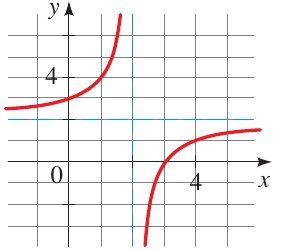
\includegraphics[width=0.5\textwidth]{fig_p10_27.png}\end{center}
\end{quote}

\begin{paso}{Paso 1 --- Intersecciones}
\textbf{Qué hago:} leo dónde la curva corta cada eje.

\textbf{¿De dónde sale?} La rama derecha cruza el eje $x$ en $x=3$; la rama izquierda cruza el eje $y$ a la altura $3$.

\textbf{¿Por qué?} Una intersección con un eje es, por definición, un punto de la gráfica sobre ese eje.
\end{paso}

\begin{paso}{Paso 2 --- Asíntotas}
\textbf{Qué hago:} identifico la recta vertical punteada y la horizontal punteada a las que se pega la curva.

\textbf{¿De dónde sale?} La gráfica sube y baja sin límite a los lados de $x=2$, y ambas ramas se aplanan hacia la recta $y=2$ cuando $|x|$ crece.

\textbf{¿Por qué?} Esa es la definición de asíntota vertical ($y\to\pm\infty$ cuando $x\to a$) y horizontal ($y\to k$ cuando $x\to\pm\infty$).
\end{paso}

\begin{resp}
Intersección $x$: $(3,0)$. \quad Intersección $y$: $(0,3)$. \quad Asíntota vertical $x=2$. \quad Asíntota horizontal $y=2$.
\end{resp}

% ===========================================================================
\subsection*{Ejercicio 29 — Leer la información de una gráfica (dos asíntotas verticales)}

\begin{quote}
\textbf{29.}
\begin{center}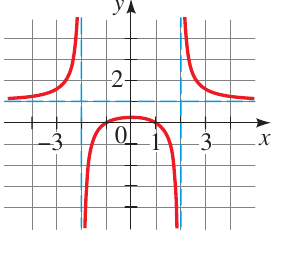
\includegraphics[width=0.5\textwidth]{fig_p10_29.png}\end{center}
\end{quote}

\begin{paso}{Paso 1 --- Intersecciones}
\textbf{Qué hago:} leo los cortes de la rama central con los ejes.

\textbf{¿De dónde sale?} La rama del medio corta el eje $x$ en $x=-1$ y $x=1$, y pasa por el eje $y$ a la altura $\tfrac14$ (un cuarto de la unidad marcada).

\textbf{¿Por qué?} Las ramas de los extremos quedan por encima de $y=1$ y nunca tocan los ejes.
\end{paso}

\begin{paso}{Paso 2 --- Asíntotas}
\textbf{Qué hago:} identifico las dos rectas verticales punteadas y la horizontal punteada.

\textbf{¿De dónde sale?} La gráfica se dispara a $\pm\infty$ junto a $x=-2$ y $x=2$, y las ramas externas se aplanan hacia $y=1$.

\textbf{¿Por qué?} Definición de asíntota vertical y horizontal, igual que en el ejercicio 27.
\end{paso}

\begin{resp}
Intersecciones $x$: $(-1,0)$ y $(1,0)$. \quad Intersección $y$: $\left(0,\tfrac14\right)$. \quad Asíntotas verticales $x=-2$ y $x=2$. \quad Asíntota horizontal $y=1$.
\end{resp}

% ===========================================================================
\subsection*{Ejercicio 31 — Asíntotas de una racional simple}

\begin{quote}
\textbf{31--42 $\blacksquare$ Asíntotas}\quad Encuentre todas las asíntotas horizontales y verticales (si las hay).

\textbf{31.} $r(x)=\dfrac{5}{x-2}$
\end{quote}

\begin{paso}{Paso 1 --- Asíntota vertical}
\textbf{Qué hago:} resuelvo $x-2=0$.

\textbf{¿De dónde sale?} Del denominador del enunciado; el numerador es la constante $5$, así que no hay factor que cancelar.

\textbf{¿Por qué?} Un cero del denominador que no se cancela con el numerador da asíntota vertical.
\[
x=2 .
\]
\end{paso}

\begin{paso}{Paso 2 --- Asíntota horizontal por comparación de grados}
\textbf{Qué hago:} comparo $n=\deg(5)=0$ con $m=\deg(x-2)=1$.

\textbf{¿De dónde sale?} De los grados del numerador y del denominador del enunciado.

\textbf{¿Por qué?} Si $n<m$ la asíntota horizontal es $y=0$.
\[
y=0 .
\]
\end{paso}

\begin{resp}
Asíntota vertical $x=2$; asíntota horizontal $y=0$.
\end{resp}

% ===========================================================================
\subsection*{Ejercicio 35 — Asíntotas con grados iguales}

\begin{quote}
\textbf{35.} $s(x)=\dfrac{6x^2+1}{2x^2+x-1}$
\end{quote}

\begin{paso}{Paso 1 --- Factorizar el denominador}
\textbf{Qué hago:} factorizo $2x^2+x-1$ por agrupación ($2x^2+2x-x-1$).

\textbf{¿De dónde sale?} Del denominador del enunciado.

\textbf{¿Por qué?} Necesito sus ceros, y el paso 1 del método exige la forma factorizada.
\[
2x^2+x-1=(2x-1)(x+1).
\]
\end{paso}

\begin{paso}{Paso 2 --- Asíntotas verticales}
\textbf{Qué hago:} anulo cada factor: $2x-1=0$ y $x+1=0$.

\textbf{¿De dónde sale?} De la factorización del paso 1.

\textbf{¿Por qué?} Ningún factor se cancela, porque $6x^2+1\ge 1>0$ para todo $x$ y por tanto no tiene ceros reales.
\[
x=\tfrac12 \quad\text{y}\quad x=-1 .
\]
\end{paso}

\begin{paso}{Paso 3 --- Asíntota horizontal}
\textbf{Qué hago:} tomo el cociente de coeficientes principales.

\textbf{¿De dónde sale?} Numerador $6x^2+1$: grado $2$, coeficiente principal $6$. Denominador $2x^2+x-1$: grado $2$, coeficiente principal $2$.

\textbf{¿Por qué?} Con $n=m$ la asíntota horizontal es $y=a_n/b_m$.
\[
y=\frac{6}{2}=3 .
\]
\end{paso}

\begin{resp}
Asíntotas verticales $x=\tfrac12$ y $x=-1$; asíntota horizontal $y=3$.
\end{resp}

% ===========================================================================
\subsection*{Ejercicio 45 — Trazar la gráfica: denominador con raíz doble}

\begin{quote}
\textbf{43--62 $\blacksquare$ Trazar gráficas de funciones racionales}\quad Encuentre los puntos de intersección y las asíntotas y luego trace una gráfica de la función racional e indique el dominio y el rango. Use una calculadora graficadora para confirmar su respuesta.

\textbf{45.} $r(x)=\dfrac{3x^2-12x+13}{x^2-4x+4}$
\end{quote}

\begin{paso}{Paso 1 --- Factorizar el denominador}
\textbf{Qué hago:} reconozco el trinomio cuadrado perfecto $x^2-4x+4$.

\textbf{¿De dónde sale?} Del denominador del enunciado: $x^2-4x+4=(x)^2-2(2)x+2^2$.

\textbf{¿Por qué?} $a^2-2ab+b^2=(a-b)^2$ (fórmula notable).
\[
r(x)=\frac{3x^2-12x+13}{(x-2)^2}.
\]
\end{paso}

\begin{paso}{Paso 2 --- Intersecciones}
\textbf{Qué hago:} busco ceros reales del numerador con el discriminante y evalúo $r(0)$.

\textbf{¿De dónde sale?} $b^2-4ac=(-12)^2-4(3)(13)=144-156=-12$; y $r(0)=\dfrac{13}{4}$.

\textbf{¿Por qué?} Discriminante negativo significa que $3x^2-12x+13$ no tiene ceros reales, así que no hay intersección con el eje $x$.
\end{paso}

\begin{paso}{Paso 3 --- Asíntotas}
\textbf{Qué hago:} tomo $x=2$ como asíntota vertical y comparo grados para la horizontal.

\textbf{¿De dónde sale?} $(x-2)^2=0$ da $x=2$, que no se cancela (el numerador no tiene ese factor); grados $2$ y $2$, coeficientes principales $3$ y $1$.

\textbf{¿Por qué?} Cero del denominador no cancelado $\Rightarrow$ asíntota vertical; $n=m \Rightarrow y=a_n/b_m$.
\[
x=2,\qquad y=\frac{3}{1}=3 .
\]
\end{paso}

\begin{paso}{Paso 4 --- Reescribir para ver el comportamiento y el rango}
\textbf{Qué hago:} completo el cuadrado en el numerador: $3x^2-12x+13=3(x-2)^2+1$.

\textbf{¿De dónde sale?} $3(x^2-4x+4)=3x^2-12x+12$, y falta $+1$ para llegar a $13$.

\textbf{¿Por qué?} Esta forma muestra la función como traslación de $y=1/x^2$, y de ahí se lee el signo y el rango.
\[
r(x)=3+\frac{1}{(x-2)^2}.
\]
\end{paso}

\begin{paso}{Paso 5 --- Comportamiento cerca de $x=2$ y rango}
\textbf{Qué hago:} concluyo $y\to+\infty$ por ambos lados de $x=2$ y $r(x)>3$ siempre.

\textbf{¿De dónde sale?} De la forma del paso 4: $(x-2)^2>0$ para $x\ne 2$, así que $\dfrac{1}{(x-2)^2}>0$.

\textbf{¿Por qué?} Sumar una cantidad estrictamente positiva a $3$ da valores mayores que $3$, y esa cantidad crece sin límite cuando $x\to 2$.
\end{paso}

\begin{center}
\begin{tikzpicture}
\begin{axis}[width=9cm,height=6.5cm,axis lines=middle,xlabel=$x$,ylabel=$y$,
  xmin=-3,xmax=7,ymin=0,ymax=12,samples=300,restrict y to domain=0:14,
  tick label style={font=\scriptsize},xtick={-2,-1,1,2,3,4,5,6},ytick={2,3,6,9,12}]
\addplot[red,very thick,domain=-3:1.66]{3+1/((x-2)^2)};
\addplot[red,very thick,domain=2.34:7]{3+1/((x-2)^2)};
\draw[blue,dashed,thick] (axis cs:2,0) -- (axis cs:2,12);
\draw[blue,dashed,thick] (axis cs:-3,3) -- (axis cs:7,3);
\end{axis}
\end{tikzpicture}
\end{center}

\begin{resp}
Sin intersección $x$; intersección $y$: $\left(0,\tfrac{13}{4}\right)$. Asíntota vertical $x=2$, asíntota horizontal $y=3$.\\
Dominio $\{x\mid x\ne 2\}$, rango $\{y\mid y>3\}=(3,\infty)$.
\end{resp}

% ===========================================================================
\subsection*{Ejercicio 53 — Trazar la gráfica: dos asíntotas verticales}

\begin{quote}
\textbf{53.} $r(x)=\dfrac{(x-1)(x+2)}{(x+1)(x-3)}$
\end{quote}

\begin{paso}{Paso 1 --- Intersecciones}
\textbf{Qué hago:} anulo cada factor del numerador y evalúo $r(0)$.

\textbf{¿De dónde sale?} $x-1=0$ y $x+2=0$; $r(0)=\dfrac{(-1)(2)}{(1)(-3)}=\dfrac{-2}{-3}$.

\textbf{¿Por qué?} La fracción vale $0$ solo donde el numerador se anula; la intersección $y$ es $r(0)$.
\[
x=1,\quad x=-2;\qquad r(0)=\frac23 .
\]
\end{paso}

\begin{paso}{Paso 2 --- Asíntotas}
\textbf{Qué hago:} anulo el denominador y comparo grados.

\textbf{¿De dónde sale?} $x+1=0$ y $x-3=0$; al desarrollar, numerador $x^2+x-2$ y denominador $x^2-2x-3$, ambos de grado $2$ con coeficiente principal $1$.

\textbf{¿Por qué?} Ningún factor es común, así que los dos ceros del denominador dan asíntotas verticales; $n=m$ da $y=1/1$.
\[
x=-1,\quad x=3;\qquad y=1 .
\]
\end{paso}

\begin{paso}{Paso 3 --- Tabla de signos con los valores frontera}
\textbf{Qué hago:} armo la tabla de signos con los ceros $-2,-1,1,3$ y un valor de prueba en cada intervalo.

\textbf{¿De dónde sale?} Los cuatro valores frontera son los ceros del numerador (pasos 1) y del denominador (paso 2).

\textbf{¿Por qué?} Una función racional solo puede cambiar de signo en un cero del numerador o del denominador.

\begin{center}
\begin{tabular}{c|ccccc}
Intervalo & $x<-2$ & $-2<x<-1$ & $-1<x<1$ & $1<x<3$ & $x>3$\\\hline
Prueba & $-3$ & $-1.5$ & $0$ & $2$ & $4$\\
$r(x)$ & $\tfrac13$ & $-\tfrac59$ & $\tfrac23$ & $-\tfrac43$ & $3.6$\\
Signo & $+$ & $-$ & $+$ & $-$ & $+$
\end{tabular}
\end{center}
\end{paso}

\begin{paso}{Paso 4 --- Comportamiento junto a las asíntotas verticales}
\textbf{Qué hago:} traduzco los signos de la tabla al lado de cada asíntota.

\textbf{¿De dónde sale?} Del paso 3: negativo a la izquierda de $x=-1$ y positivo a su derecha; negativo a la izquierda de $x=3$ y positivo a su derecha.

\textbf{¿Por qué?} Junto a una asíntota vertical $|y|$ crece sin límite, y el signo del intervalo dice hacia dónde.
\[
y\to-\infty \text{ si } x\to-1^-,\quad y\to+\infty \text{ si } x\to-1^+;\qquad
y\to-\infty \text{ si } x\to3^-,\quad y\to+\infty \text{ si } x\to3^+.
\]
\end{paso}

\begin{paso}{Paso 5 --- Rango: la gráfica cruza la asíntota horizontal}
\textbf{Qué hago:} resuelvo $r(x)=1$ para ver si el valor $1$ se alcanza.

\textbf{¿De dónde sale?} $\dfrac{x^2+x-2}{x^2-2x-3}=1 \Rightarrow x^2+x-2=x^2-2x-3 \Rightarrow 3x=-1$.

\textbf{¿Por qué?} Una asíntota horizontal sí puede cruzarse; solo describe el comportamiento para $|x|$ grande. Como $x=-\tfrac13$ está en el dominio, $y=1$ se alcanza y el rango es todo $\mathbb{R}$.
\end{paso}

\begin{center}
\begin{tikzpicture}
\begin{axis}[width=10cm,height=7cm,axis lines=middle,xlabel=$x$,ylabel=$y$,
  xmin=-6,xmax=8,ymin=-6,ymax=7,samples=400,restrict y to domain=-9:10,
  tick label style={font=\scriptsize},xtick={-5,-4,-3,-2,-1,1,2,3,4,5,6,7},ytick={-4,-2,1,3,5}]
\addplot[red,very thick,domain=-6:-1.06]{((x-1)*(x+2))/((x+1)*(x-3))};
\addplot[red,very thick,domain=-0.94:2.72]{((x-1)*(x+2))/((x+1)*(x-3))};
\addplot[red,very thick,domain=3.42:8]{((x-1)*(x+2))/((x+1)*(x-3))};
\draw[blue,dashed,thick] (axis cs:-1,-6) -- (axis cs:-1,7);
\draw[blue,dashed,thick] (axis cs:3,-6) -- (axis cs:3,7);
\draw[blue,dashed,thick] (axis cs:-6,1) -- (axis cs:8,1);
\end{axis}
\end{tikzpicture}
\end{center}

\begin{resp}
Intersecciones $x$: $(-2,0)$ y $(1,0)$; intersección $y$: $\left(0,\tfrac23\right)$. Asíntotas verticales $x=-1$ y $x=3$; asíntota horizontal $y=1$.\\
Dominio $\{x\mid x\ne -1,\ x\ne 3\}$, rango $\mathbb{R}$.
\end{resp}

% ===========================================================================
\subsection*{Ejercicio 63 — Función racional con hueco}

\begin{quote}
\textbf{63--68 $\blacksquare$ Funciones racionales con huecos}\quad Encuentre los factores que son comunes en el numerador y en el denominador. Luego determine las intersecciones y las asíntotas y trace una gráfica de la función racional. Indique el dominio y el rango de la función.

\textbf{63.} $r(x)=\dfrac{x^2+4x-5}{x^2+x-2}$
\end{quote}

\begin{paso}{Paso 1 --- Factorizar y detectar el factor común}
\textbf{Qué hago:} factorizo los dos trinomios y cancelo el factor repetido.

\textbf{¿De dónde sale?} $x^2+4x-5=(x+5)(x-1)$ ($5\cdot(-1)=-5$, $5+(-1)=4$) y $x^2+x-2=(x+2)(x-1)$ ($2\cdot(-1)=-2$, $2+(-1)=1$).

\textbf{¿Por qué?} La cancelación es válida solo donde el factor no es cero, así que hay que arrastrar la restricción $x\ne 1$.
\[
r(x)=\frac{(x+5)(x-1)}{(x+2)(x-1)}=\frac{x+5}{x+2},\qquad x\ne 1 .
\]
\end{paso}

\begin{paso}{Paso 2 --- Hueco}
\textbf{Qué hago:} calculo el valor que tendría la función simplificada en $x=1$.

\textbf{¿De dónde sale?} $\dfrac{1+5}{1+2}=\dfrac63=2$.

\textbf{¿Por qué?} El factor común $x-1$ se cancela, así que en $x=1$ no hay asíntota sino un hueco en el punto $(1,2)$.
\end{paso}

\begin{paso}{Paso 3 --- Intersecciones y asíntotas}
\textbf{Qué hago:} anulo $x+5$, evalúo $r(0)$, anulo $x+2$ y comparo grados.

\textbf{¿De dónde sale?} $x+5=0$ da $x=-5$; $r(0)=\dfrac{5}{2}$; $x+2=0$ da $x=-2$; en la forma original ambos grados son $2$ con coeficiente principal $1$.

\textbf{¿Por qué?} Ceros del numerador $\Rightarrow$ intersecciones $x$; cero del denominador no cancelado $\Rightarrow$ asíntota vertical; $n=m \Rightarrow y=1$.
\[
x=-5;\quad r(0)=\tfrac52;\qquad x=-2;\qquad y=1 .
\]
\end{paso}

\begin{paso}{Paso 4 --- Dominio y rango}
\textbf{Qué hago:} excluyo $-2$ y $1$ del dominio, y $1$ y $2$ del rango.

\textbf{¿De dónde sale?} Del denominador original $(x+2)(x-1)$; y de $\dfrac{x+5}{x+2}=1+\dfrac{3}{x+2}$, que nunca vale $1$, más el hueco de altura $2$ del paso 2.

\textbf{¿Por qué?} El dominio se toma de la expresión original, no de la simplificada; y el valor $2$ solo se alcanzaría en $x=1$, que está excluido.
\end{paso}

\begin{center}
\begin{tikzpicture}
\begin{axis}[width=9cm,height=6.5cm,axis lines=middle,xlabel=$x$,ylabel=$y$,
  xmin=-9,xmax=5,ymin=-5,ymax=7,samples=300,restrict y to domain=-8:10,
  tick label style={font=\scriptsize},xtick={-8,-6,-5,-4,-2,1,2,4},ytick={-4,-2,1,2,4,6}]
\addplot[red,very thick,domain=-9:-2.55]{(x+5)/(x+2)};
\addplot[red,very thick,domain=-1.45:5]{(x+5)/(x+2)};
\draw[blue,dashed,thick] (axis cs:-2,-5) -- (axis cs:-2,7);
\draw[blue,dashed,thick] (axis cs:-9,1) -- (axis cs:4,1);
\node[circle,draw=red,fill=white,inner sep=1.6pt] at (axis cs:1,2) {};
\end{axis}
\end{tikzpicture}
\end{center}

\begin{resp}
Factor común: $x-1$, que produce un hueco en $(1,2)$.\\
Intersección $x$: $(-5,0)$; intersección $y$: $\left(0,\tfrac52\right)$. Asíntota vertical $x=-2$; asíntota horizontal $y=1$.\\
Dominio $\{x\mid x\ne -2,\ x\ne 1\}$, rango $\{y\mid y\ne 1,\ y\ne 2\}$.
\end{resp}

% ===========================================================================
\subsection*{Ejercicio 69 — Asíntota inclinada}

\begin{quote}
\textbf{69--76 $\blacksquare$ Asíntotas inclinadas}\quad Encuentre la asíntota inclinada, las asíntotas verticales y trace una gráfica de la función.

\textbf{69.} $r(x)=\dfrac{x^2}{x-2}$
\end{quote}

\begin{paso}{Paso 1 --- Asíntota vertical y ausencia de horizontal}
\textbf{Qué hago:} anulo $x-2$ y comparo grados.

\textbf{¿De dónde sale?} $x-2=0$ da $x=2$; el numerador $x^2$ tiene grado $2$ y el denominador grado $1$.

\textbf{¿Por qué?} $x^2$ no tiene el factor $x-2$, así que $x=2$ es asíntota vertical; y con $n>m$ no hay asíntota horizontal.
\end{paso}

\begin{paso}{Paso 2 --- División larga para la asíntota inclinada}
\textbf{Qué hago:} divido $x^2$ entre $x-2$.

\textbf{¿De dónde sale?} $x^2=(x-2)(x+2)+4$, porque $(x-2)(x+2)=x^2-4$ y falta $+4$.

\textbf{¿Por qué?} Cuando el grado del numerador es uno más que el del denominador, el cociente $ax+b$ de la división es la asíntota inclinada, ya que el término $\frac{4}{x-2}$ se hace despreciable para $|x|$ grande.
\[
r(x)=x+2+\frac{4}{x-2}\;\Longrightarrow\; y=x+2 .
\]
\end{paso}

\begin{paso}{Paso 3 --- Intersecciones y signo}
\textbf{Qué hago:} anulo el numerador y armo la tabla de signos con los valores frontera $0$ y $2$.

\textbf{¿De dónde sale?} $x^2=0$ da $x=0$ (única intersección, y también la intersección $y$); pruebas $x=-1$, $x=1$, $x=3$.

\textbf{¿Por qué?} $x^2\ge 0$ siempre, así que el signo lo decide solo $x-2$: negativo para $x<2$ y positivo para $x>2$.
\[
y\to-\infty \text{ si } x\to 2^-,\qquad y\to+\infty \text{ si } x\to 2^+ .
\]
\end{paso}

\begin{center}
\begin{tikzpicture}
\begin{axis}[width=9.5cm,height=7cm,axis lines=middle,xlabel=$x$,ylabel=$y$,
  xmin=-6,xmax=9,ymin=-12,ymax=20,samples=400,restrict y to domain=-16:26,
  tick label style={font=\scriptsize},xtick={-4,-2,2,4,6,8},ytick={-8,-4,4,8,12,16}]
\addplot[red,very thick,domain=-6:1.6]{(x^2)/(x-2)};
\addplot[red,very thick,domain=2.35:9]{(x^2)/(x-2)};
\draw[blue,dashed,thick] (axis cs:2,-12) -- (axis cs:2,20);
\addplot[blue,dashed,thick,domain=-6:9,samples=2]{x+2};
\end{axis}
\end{tikzpicture}
\end{center}

\begin{resp}
Asíntota inclinada $y=x+2$; asíntota vertical $x=2$; no hay asíntota horizontal.\\
Única intersección: el origen $(0,0)$.
\end{resp}

% ===========================================================================
\subsection*{Ejercicio 87 — Aplicación: crecimiento poblacional}

\begin{quote}
\textbf{87. Crecimiento poblacional}\quad Suponga que la población de conejos de la granja del Sr. Jenkin sigue la fórmula
\[
p(t)=\frac{3000t}{t+1}
\]
donde $t\ge 0$ es el tiempo (en meses) desde principios de año.
\begin{enumerate}[label=\emph{\alph*}\,), leftmargin=*]
\item Trace una gráfica de la población de conejos.
\item ¿Qué le ocurre finalmente a la población de conejos?
\end{enumerate}
\end{quote}

\begin{paso}{Paso 1 --- Dominio del modelo}
\textbf{Qué hago:} restrinjo el dominio a $t\ge 0$.

\textbf{¿De dónde sale?} Del enunciado, que define $t\ge 0$ como meses desde principios de año.

\textbf{¿Por qué?} El único cero del denominador es $t=-1$, que queda fuera del dominio; por eso la gráfica no tiene asíntota vertical.
\end{paso}

\begin{paso}{Paso 2 --- Puntos de referencia}
\textbf{Qué hago:} evalúo $p$ en algunos valores para tener la forma de la curva.

\textbf{¿De dónde sale?} De sustituir en $p(t)=\dfrac{3000t}{t+1}$.

\textbf{¿Por qué?} El paso 5 del método pide puntos adicionales para completar el trazado.
\[
p(0)=0,\quad p(1)=1500,\quad p(5)=2500,\quad p(9)=2700 .
\]
\end{paso}

\begin{paso}{Paso 3 --- Asíntota horizontal}
\textbf{Qué hago:} comparo grados: numerador $3000t$ y denominador $t+1$, ambos de grado $1$.

\textbf{¿De dónde sale?} Coeficientes principales $3000$ y $1$.

\textbf{¿Por qué?} Con $n=m$ la asíntota horizontal es $y=a_n/b_m$, y describe el valor al que tiende la población cuando $t$ crece.
\[
p=\frac{3000}{1}=3000 .
\]
\end{paso}

\begin{center}
\begin{tikzpicture}
\begin{axis}[width=10cm,height=6cm,axis lines=middle,xlabel=$t$ (meses),ylabel=$p$,
  xmin=0,xmax=30,ymin=0,ymax=3600,samples=200,
  tick label style={font=\scriptsize},xtick={5,10,15,20,25,30},ytick={1000,2000,3000}]
\addplot[red,very thick,domain=0:30]{3000*x/(x+1)};
\draw[blue,dashed,thick] (axis cs:0,3000) -- (axis cs:30,3000);
\end{axis}
\end{tikzpicture}
\end{center}

\begin{resp}
\emph{a}) Curva creciente que arranca en $(0,0)$ y se aplana bajo la recta $p=3000$.\\
\emph{b}) La población se acerca cada vez más a $3000$ conejos sin llegar a alcanzarlos, porque $p=3000$ es la asíntota horizontal del modelo.
\end{resp}

\end{document}
